\subsection{Motion Extraction}\label{sec:motion_extraction}
After specifying the control points, we track their positions throughout the video.
A na\"{i}ve approach would be to track each control point individually using standard point tracking methods, e.g., KLT point tracker~\cite{yilmaz2006object}. 
However, these methods may fail for some points that are hard to track, e.g., points specified in textureless regions, resulting in drifting. Used as hard constraints, these drifted points will later distort the sketch shape in the final animation.
Given that automatic tracking failure may always occur no matter how robust the underlying algorithm is,  
we employ an interactive tracking procedure. We first adopt the dynamic-programming-based trajectory optimization framework~\cite{Amberg:2011,Buchanan:2006} to track individual points, which is quite efficient and can provide near real-time feedback to the user. 
When tracking failure occurs, the user only needs to modify the tracking position of a failed point on a particular frame, and this method can use it as a hard constraint to globally refine the whole trajectory. Therefore, the user can quickly refine the tracking results by only editing a few frames.

Specifically, the tracking algorithm optimizes the following energy for each feature trajectory:
\begin{equation}\label{eq:tracking}
E_{tr}(\textbf{x}) = \sum_t\lambda_d d(\textbf{x}_t, \textbf{x}_{t-1})+\lambda_u u(\textbf{p}_t,\textbf{p}_{t-1})+\min_k(a(\textbf{p}_t,\textbf{c}_k)),
\end{equation}
\ca{where $ \textbf{x}_t $ represents the position of the control point on frame $t$, and $ \textbf{p}_t $ denotes the feature descriptor of the image patch centered at $\textbf{x}_t$. The energy includes three parts. The velocity term $ d(\cdot)=\|\textbf{x}_t - \textbf{x}_{t-1}\|^2_2 $ and update penalty term $ u(\cdot)=\|\textbf{p}_t - \textbf{p}_{t-1}\|^2_2 $ measure the motion intensity and appearance variation between two consecutive frames, to achieve a smooth motion and appearance transition. The third term $ a(\cdot) = \|\textbf{p}_t - \textbf{c}_k\|^2_2 $ is a measure of the appearance deviation from the user-specified control point locations $ \{\textbf{c}_k\} $. User may manually specifies two or more control point positions at different frames. We measure the appearance energy of points at other frames using $ \min_k(a(\textbf{p}_t,\textbf{c}_k)) $, so that they should match at least one of these $ k $ control points. }
The optimization is mainly divided into two stages: preprocessing using k-d tree and trajectory optimization based on dynamic programming. More details of this method can be found in~\cite{Amberg:2011,Buchanan:2006}.

Built upon this algorithmic framework, we further improve the tracking method by addressing two common problems that lead to drifting: occlusion and ambiguity. These additional components, as detailed in the next two sections, allow our tracking method to perform more reliably than previous ones on tracking complex object motion with topology changes. 


\subsubsection{Occlusion Handling}
% \hongbo{Qingkun: check if this part is our contribution or not}
Occlusion has been considered by many existing automatic tracking methods. However, it still leads to serious drifting in difficult cases. There exists no good user interface for correcting drifting other than manually editing results frame by frame.
Following~\cite{Amberg:2011}, we modify the graph used for dynamic programming by adding extra edges from each control point to all points on the next few frames. When occlusion happens, the optimization favors a trajectory that passes through the extra edges, thus skipping a few frames where occlusion occurs in.
In our system, the skipped/occluded part of the trajectory is interpolated using Hermite interpolation for smooth animation. 
%as tracking errors of individual control points often lead to significant distortion of the sketch image. Such an example is shown in Fig.~\ref{fig:distortion}, where \ca{XXX}


\subsubsection{Ambiguity Handling}\label{sec:ambi}

Another source of drifting is ambiguity, i.e., when two or more tracking points with similar appearance get close to each other. An example is shown in Fig.~\ref{fig:ambiguityhandling}. When the two legs of the tiger cross, the two control points become too close to each other, and they end up tracking the same image feature going forward, resulting in a collide.  

To solve this problem, we propose a new energy minimization method to jointly optimize the tracking results of multiple points together. 
The main idea of this method is that instead of tracking a single trajectory for each point individually, we first generate a set of trajectories for each control point as candidates, and then employ a global optimization approach to select the best one for each point, by jointly considering multiple points together.

{\bf Candidate Trajectories.}
Given all control points on a keyframe, we first compute the appearance similarity between any two points, based on the image patch color distance centered around them (we use $9\times 9$ patches). We then group points into several sets, each containing the points that have similar appearance. Denote one such set  as $S=\{\textbf{x}^1,...,\textbf{x}^n\}$. For each point $\textbf{x}^i$,
we apply the method proposed in~\cite{chondrogiannis2015alternative} to compute a set of candidate tracking trajectories. This method has two major parameters: (1) the maximum overlap between any two candidate trajectories, which we set as $T/4$, where $T$ is the total number of frames; and (2) a tracking cost threshold. We then sort the candidates based on their tracking costs (computed in Eq.~\ref{eq:tracking}).

{\bf Trajectory Optimization.}
In the next step, we find the best trajectory for each point by  jointly optimizing over multiple tracking points.
This can be formulated as the following energy minimization problem:
\begin{equation}\label{key}
\arg \min \sum_{i}E(\textbf{x})= \arg \min \sum_{i} (E_{tr}(\textbf{x}) + \beta \sum_{j \neq i} E_o(\textbf{x}_{i}, \textbf{x}_{j})),
\end{equation}
where the tracking energy $ E_{tr}(\textbf{x}) $ is measured by Eq.~\ref{eq:tracking}. $ E_o({\textbf{x}_{i}, \textbf{x}_{j}}) $ is defined as the normalized duration of the overlapping portion of the two trajectories. Intuitively, this term prevents two similar control points to collapse into a single one, in which case the overlapping portion of the two trajectories will be large. 

We use a greedy algorithm to minimize this energy. 
We first initialize the solution by choosing the trajectory that has the minimal tracking energy for each point. We then find the point that has the largest total energy according to Eq.~\ref{key}, and select another candidate trajectory that can best minimize this energy. We repeat this process until the total energy cannot be further reduced. 

\begin{figure}
	\centering
	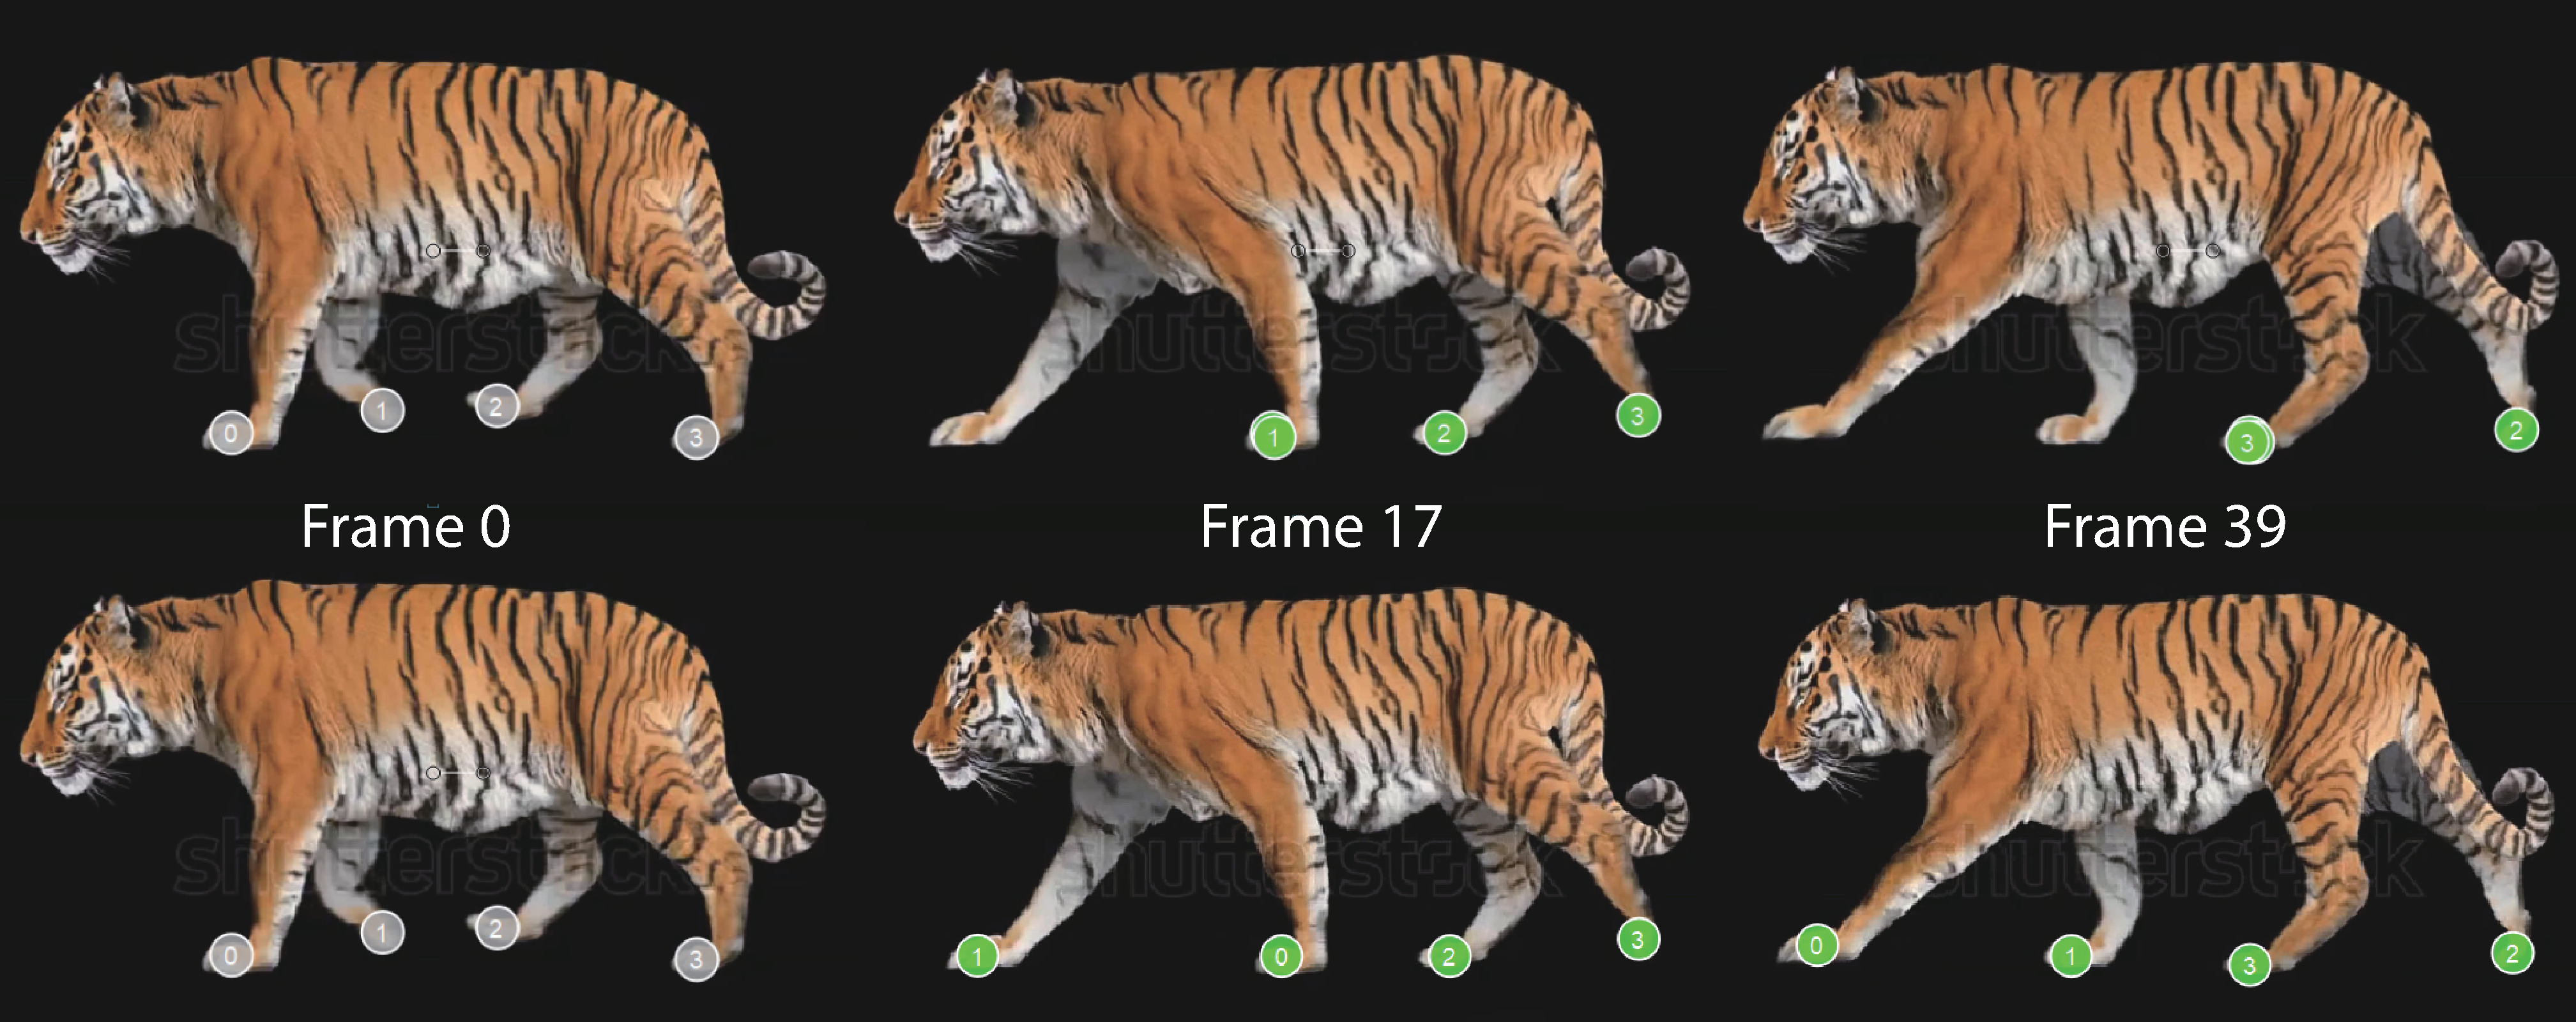
\includegraphics[width=\linewidth]{images/ambiguityhandling2}
	\caption{Solving tracking ambiguity using multi-track optimization. Top: four control points defined on the four legs collide when the legs cross, due to appearance ambiguity. Bottom: our new tracking method proposed in Sec.~\ref{sec:ambi} can effectively prevent such cases.}
	\label{fig:ambiguityhandling}
\end{figure}


%Then 
%compute the overlapping ratio between each point pair $ (i, j) $ based on current optimal . We let the ratio as .
%Denote the optimal trajectory candidate of each point as $ \textbf{p}^*_i $. We first initialize it as $ \textbf{p}_{i1} $, which has minimum tracking cost, but may have large overlapping with other points.
%\paragraph{Overlapping Detection}
%%Before tracking, we first compute the similarity between all objects that are specified manually by the user based on patch descriptor (we use SURF feature in our implementation). 
%
%Given a set of similar points, they may overlaps with each other during the tracking. We first obtain their trajectories $ \{\textbf{p}\} $ by tracking each point individually. Then for each pair of trajectory $ \textbf{p}^a $ and $ \textbf{p}^b $ of two keypoint $ a $ and $ b $  of this set, we compute their closeness at each frame by: 
%\begin{array}\label{eq:closeness}
%C(p^a_f, p^b_f) = \alpha\lVert p^a_f-p^b_f \rVert^2_2 + (1-v^a_f \cdot v^b_f),
%\end{equation}
%where $ v^a_f$ and $ v^b_f $ are the normalized vector of $ \overrightarrow{p^a_{f-1}p^a_f} $ and $ \overrightarrow{p^b_{f-1}p^b_f} $. The first term represents their Euclidean distance and the second term represents their direction consistency. 
%The equation implies that the two trajectories are close only when their distance is small and their direction is same.
%When $ C(p^a_f, p^b_f) \leq \epsilon$, the two trajectories are flagged as overlapping at the $ f $th frame.
%
%Based on this measurement, we count the overlapping frames, which is denoted as $ C(p^a, p^b) $.
%%Based on this measurement, we denote the overlapping time interval $ I=[n, m] $ when overlapping happens between $ n $th and $ m $th frame. To tolerate instant overlapping, we only considers the overlapping intervals with length larger than 3, i.e. $ m - n>=3 $.
%$ \alpha $ and $ \epsilon $ are set 0.02 and 3.0 in our implementation.
%Finally, we can obtain a set of overlapping intervals between each pair of trajectories. 
%
%%Then an overlapping detection is run between each similar object pair after we obtained the trajectory using graph tracking for each object. Given one point pair $ p_i,q_i $ of the two trajectories $ \textbf{p},\textbf{q} $, , the intesection parts are detected based on the following equation:
%%\begin{equation}\label{key}
%%f(p_i, q_i) = \alpha\lVert p_i-q_i \rVert^2_2 + (1-u_i \cdot v_i),
%%\end{equation}
%%where $ u_i$ and $ v_i $ is the normalized vector of $ \overrightarrow{p_{i-1}p_i} $ and $ \overrightarrow{q_{i-1}q_i} $. It means two trajectories overlapps at $ p_i $ and $ q_i $ only when their distance is small and their direction is similar.  $ \alpha = 0.02 $ in our implementation.
%%Then when $ f(p_i,q_i) \leq 3$, it means the two trjactories $ \textbf{p} $ and $ \textbf{q} $ overlap at the $ i $th frame.
%
%\paragraph{Overlapping Removal}
%Next we run the overlapping removal for each of the overlapping intervals one by one in time order.
%First, for each similar point set, we sort all overlapping intervals by their starting time. Then the intervals will be removed according to this order.
%
%Given the first interval $ I=[n, m] $, we modify the edge weight of keypoint $ a $'s graph in the overlapping interval by
%%Because we assume that there is no long common consecutive trajectory parts shared by two objects, we need to remove the overlapping when a long sequence of overlapping frames exists.
%
%\begin{equation}
%\begin{array}{rcl}
%w(e) & = & +\infty \text{ if }C(e) < \epsilon\\
%C(e) & = & \alpha\lVert p^a_f-x_f \rVert^2_2 + (1-v^a \cdot v^e) 
%\end{array}
%\end{equation}
%
%$ e_f=(x_f,y_g) $ is an edge in keypoint $ b $'s graph from the $ f $th to the $ g $th frame, $ v^e $ is the normalized vector of $ \overrightarrow{xy} $ and $ v^a $ is the normalized vector of $ \overrightarrow{p^a_f p^a_g} $.
%The reweighting makes sure that there is no tracking path passing though the overlapping parts. 
%Then we update the part of $ a $'s trajectory, which starts from frame $ m $ based on $ a $'s reweighted graph to the end. Denote the new trajectory as $ \textbf{q}^a $. We also reweight keypoint $ b $ graph using similar way and update $ b $'s trajectory, which is denoted as $ \textbf{q}^b $.
%If the cost of $ \textbf{q}^a $ is smaller than $ \textbf{q}^b $, we set the trajectory of $ a $ as $ \textbf{q}^a $ and keep the $ b $'s trajectory unchanged, i.e. the two trajectories become $ \textbf{q}^a, \textbf{p}^b $.
%Otherwise, we set $ b $'s trajectory as $ \textbf{q}^b $ and keep $ a $'s trajectory unchanged. Their trajectories become $ \textbf{p}^a, \textbf{q}^b $. Obviously, because of the reweighting scheme, there is no overlapping between their new trajectories in both scenarios during the interval $ I=[n, m] $. Therefore, one overlapping interval is removed. 
%
%We recompute the overlapping status among the new trajectory set and obtain the new first interval $ I'=[n', m'] $. 
%Note that $ [n,m] $ is the first appeared overlapping interval before and the second pass does not change the positions of the trajectories between the interval $ [1,n] $. Therefore, the overlapping status between interval $ [1,n] $ does not change, i.e. no overlapping exists in $ [1,n] $ and $ n'> n $. It ensures that the overlapping intervals can be removed one by one according to the time order.